% ----------------------------------------------------
\begin{frame}
  \titlepage
\end{frame}
% ----------------------------------------------------
\note{Introduccion a la sesion sobre desarrollo economico. Conectar con la sesion anterior sobre finanzas internacionales: hemos visto como fluyen el dinero y el capital, ahora nos preguntamos por que ese capital y esas oportunidades no se distribuyen de forma igualitaria entre paises. El desarrollo economico es quizas el gran reto de la politica mundial: miles de millones de personas viven en la pobreza, y las diferencias entre paises ricos y pobres son enormes. Hoy exploraremos por que existen esas diferencias, que factores las explican, y que estrategias se han intentado para cerrar la brecha.}

% ----------------------------------------------------
\begin{frame}
\frametitle{Hoy}
\centering
\vspace{1.5em}
\begin{itemize}
  \setlength{\itemsep}{10pt}
  \item El rompecabezas: \textquestiondown por qu\'{e} unos pa\'{i}ses son ricos y otros pobres?
  \item Factores dom\'{e}sticos: geograf\'{i}a, intereses y recursos
  \item Instituciones y desarrollo
  \item El entorno internacional: colonialismo y comercio
  \item Estrategias de desarrollo: ISI, EOI y el Consenso de Washington
  \item \textquestiondown Ayuda o comercio?
\end{itemize}
\end{frame}
% ----------------------------------------------------
\note{Seis bloques en la sesion. Empezar con el rompecabezas (por que la diferencia entre paises ricos y pobres) para motivar la pregunta. Luego factores domesticos (geografia, intereses, recursos) e instituciones como explicaciones centrales. Despues el entorno internacional (colonialismo, terminos de intercambio, instituciones sesgadas). Las estrategias de desarrollo (ISI, EOI, Consenso de Washington) muestran las respuestas politicas a lo largo del tiempo. Cerrar con el debate ayuda vs. comercio, que conecta todo. Tiempo estimado: 10 min rompecabezas, 15 min factores domesticos, 10 min instituciones, 15 min entorno internacional, 15 min estrategias, 10 min debate final. Conectar con la sesion anterior sobre finanzas: hoy vemos el otro lado de la moneda --- por que el capital y las oportunidades no se distribuyen de forma igualitaria.}

% ====================================================
\section{El rompecabezas del desarrollo}
% ====================================================

% ----------------------------------------------------
\begin{transitionframe}
El rompecabezas del desarrollo
\end{transitionframe}
% ----------------------------------------------------
\note{}

% ----------------------------------------------------
\begin{frame}[plain]
  \begin{tikzpicture}[remember picture, overlay]
    \node[at = (current page.center), yshift = 0cm] (cover) {%
      \includegraphics[keepaspectratio, height=\paperheight]{../img/poverty_comparison.jpg}};
  \end{tikzpicture}
\end{frame}
% ----------------------------------------------------
% IMAGE NEEDED: poverty_comparison.jpg -- imagen de contraste entre pobreza extrema (p.ej., barrio marginal en un pais en desarrollo) y riqueza urbana moderna (p.ej., skyline de una gran ciudad); side by side o composicion visual que muestre la desigualdad global
\note{Imagen de apertura. La desigualdad global es el punto de partida de esta sesion. Un nino nacido en Noruega tiene una esperanza de vida de 83 anos, acceso a educacion universal y sanidad publica. Un nino nacido en Sierra Leona tiene una esperanza de vida de 54 anos y una probabilidad significativa de no llegar a los 5 anos. Estas diferencias no son naturales ni inevitables: son el resultado de procesos historicos, politicos y economicos que vamos a explorar hoy.}

% ----------------------------------------------------
\begin{frame}
\frametitle{El rompecabezas}
\centering

\begin{itemize}
  \item \textquestiondown Por qu\'{e} unos pa\'{i}ses son ricos y otros pobres?
  \vspace{4pt}
  \item<2-> Las diferencias son \textbf{enormes}:
  \begin{itemize}
    \item PIB per c\'{a}pita de EE.UU.: $\sim$\textbf{80.000\$}
    \item PIB per c\'{a}pita de Zambia: $\sim$\textbf{1.300\$}
    \item Ratio $\approx$ 60:1
  \end{itemize}
  \vspace{4pt}
  \item<3-> Pero la pobreza global \textbf{ha disminuido}:
  \begin{itemize}
    \item 1981: \textbf{52\%} de la poblaci\'{o}n mundial en pobreza extrema
    \item 2013: \textbf{11\%}
    \item Gran parte del avance: China e India
  \end{itemize}
  \vspace{4pt}
  \item<4-> A\'{u}n as\'{i}, \alert{cientos de millones} siguen en la pobreza
\end{itemize}

\end{frame}
% ----------------------------------------------------
\note{El rompecabezas del desarrollo es quizas la pregunta mas importante de la economia politica internacional. Las diferencias de renta entre paises son mucho mayores que las diferencias dentro de cada pais. La buena noticia es que la pobreza extrema ha disminuido drasticamente en las ultimas decadas, pero esto se debe en gran parte a China (que saco a mas de 800 millones de personas de la pobreza entre 1980 y 2015) y a India. En Africa subsahariana, la mejora ha sido mucho mas lenta. El punto clave: no hay una sola explicacion para estas diferencias. La sesion explorara multiples factores: geografia, instituciones, intereses politicos, el legado colonial, y las estrategias de desarrollo adoptadas.}

% ----------------------------------------------------
\begin{frame}
\frametitle{Zambia vs.\ Corea del Sur}
\centering
\vspace{0.5em}

{\footnotesize
\begin{adjustbox}{width=\textwidth}
\begin{tabular}{>{\bfseries}p{3.2cm} p{3cm} p{3cm}}
 & \textbf{\textcolor{accent}{Zambia}} & \textbf{\textcolor{accent2}{Corea del Sur}} \\[6pt]
\hline
PIB p.c.\ en 1964 & $\sim$1.500\$ & $\sim$1.500\$ \\[5pt]
PIB p.c.\ hoy & $\sim$1.300\$ & $\sim$35.000\$ \\[5pt]
Independencia & 1964 (de R.\ Unido) & 1945 (de Jap\'{o}n) \\[5pt]
Recursos naturales & Cobre (abundante) & Escasos \\[5pt]
Estrategia & Dependencia del cobre & Industrializaci\'{o}n exportadora \\[5pt]
Resultado & Estancamiento & ``Milagro asi\'{a}tico'' \\[5pt]
\end{tabular}
\end{adjustbox}
}

\vspace{8pt}
\onslide<2->{\small En 1964, ambos pa\'{i}ses eran pr\'{a}cticamente \textbf{iguales} en renta per c\'{a}pita.\\ \alert{\textquestiondown Qu\'{e} explica la divergencia?}}

\end{frame}
% ----------------------------------------------------
\note{El caso de Zambia y Corea del Sur es el ejemplo clasico del libro de FLS para motivar la pregunta del desarrollo.
\begin{itemize}
  \item En 1964, las perspectivas de Zambia parecian mucho mejores que las de Corea del Sur: Zambia era rica en cobre, su presidente Kaunda era respetado. Corea del Sur no tenia recursos, estaba gobernada por una dictadura militar despreciada, y dependia de ayuda americana que se estaba recortando.
  \item Hoy, Corea del Sur tiene un PIB per capita de unos 35.000 dolares (comparable a Francia), esperanza de vida de 82 anos, y es miembro de la OCDE desde 1996. Zambia tiene un PIB per capita inferior a 1.200 dolares, esperanza de vida de 61 anos, y dos tercios de la poblacion bajo el umbral de pobreza.
  \item La divergencia no se explica por la geografia ni por los recursos, sino por las politicas, las instituciones, y el entorno internacional. Este caso nos acompana toda la sesion como hilo conductor.
\end{itemize}}

% ----------------------------------------------------
\begin{frame}[plain]
  \begin{tikzpicture}[remember picture, overlay]
    \node[at = (current page.center), yshift = 0cm] (cover) {%
      \includegraphics[keepaspectratio, height=\paperheight]{../img/zambia_korea.jpg}};
  \end{tikzpicture}
\end{frame}
% ----------------------------------------------------
% IMAGE NEEDED: zambia_korea.jpg -- composicion visual comparando Zambia y Corea del Sur; por ejemplo, lado izquierdo una zona rural o minera de Zambia, lado derecho el skyline moderno de Seul; o un grafico que muestre la divergencia del PIB per capita desde 1964
\note{Imagen que ilustra la divergencia. En 1964, las capitales de ambos paises no eran tan diferentes. Hoy, Seul es una de las ciudades mas modernas del mundo, con Samsung, Hyundai, y una industria tecnologica puntera. Lusaka sigue siendo una ciudad con enormes desafios de infraestructura y pobreza. La pregunta es: que paso entre 1964 y hoy que explique esta divergencia tan radical entre dos paises que partian de una situacion similar.}

% ====================================================
\section{Factores dom\'{e}sticos}
% ====================================================

% ----------------------------------------------------
\begin{transitionframe}
Factores dom\'{e}sticos
\end{transitionframe}
% ----------------------------------------------------
\note{}

% ----------------------------------------------------
\begin{frame}
\frametitle{Geograf\'{i}a y desarrollo}
\centering

\begin{itemize}
  \item \textbf{Sachs (2001):} la geograf\'{i}a importa
  \begin{itemize}
    \item Pa\'{i}ses tropicales: enfermedades (malaria), baja productividad agr\'{i}cola
    \item Pa\'{i}ses sin litoral (\textit{landlocked}): costes de transporte elevados
    \item Climas templados: ventajas agr\'{i}colas hist\'{o}ricas
  \end{itemize}
  \vspace{8pt}
  \item<2-> \textbf{Pero la geograf\'{i}a no es destino:}
  \begin{itemize}
    \item Singapur: tropical, sin recursos, isla diminuta $\rightarrow$ renta alt\'{i}sima
    \item Bolivia: riqueza mineral enorme $\rightarrow$ pobreza persistente
    \item Botsuana vs.\ Zambia: similar geograf\'{i}a, resultados muy distintos
  \end{itemize}
  \vspace{8pt}
  \item<3-> La geograf\'{i}a puede \textbf{condicionar}, pero no \alert{determinar} el desarrollo
\end{itemize}

\end{frame}
% ----------------------------------------------------
\note{La hipotesis geografica tiene una larga tradicion en las explicaciones del desarrollo (Montesquieu ya la proponia en el siglo XVIII). Jeffrey Sachs es su defensor mas conocido hoy: argumenta que los paises tropicales enfrentan desventajas reales (enfermedades endemicas como la malaria que reducen la productividad laboral, suelos menos fertiles para la agricultura cerealista, costes de refrigeracion). Los paises sin litoral (landlocked) como Bolivia, Etiopia o Chad tienen costes de transporte mucho mas altos para acceder a los mercados internacionales. Sin embargo, la geografia no puede explicar la totalidad de las diferencias: Singapur es tropical y es uno de los paises mas ricos del mundo; Botsuana y Zambia comparten una frontera y una posicion geografica similar, pero sus trayectorias de desarrollo han sido muy distintas.}

% ----------------------------------------------------
\begin{frame}
\frametitle{Intereses dom\'{e}sticos}
\centering

\begin{itemize}
  \item Grupos poderosos pueden \textbf{bloquear} el desarrollo si les beneficia el \textit{statu quo}
  \vspace{5pt}
  \item<2-> \textbf{Ejemplo: \'{A}frica subsahariana}
  \begin{itemize}
    \item \'{E}lites urbanas con poder pol\'{i}tico
    \item Precios agr\'{i}colas artificialmente bajos $\rightarrow$ subvenciones urbanas
    \item Resultado: sector rural empobrecido, sin incentivos para producir
  \end{itemize}
  \vspace{5pt}
  \item<3-> \textbf{Ejemplo: Latinoam\'{e}rica}
  \begin{itemize}
    \item Oligarqu\'{i}as terratenientes bloquearon reformas agrarias y educativas
    \item Alta desigualdad $\rightarrow$ baja inversi\'{o}n en bienes p\'{u}blicos
  \end{itemize}
  \vspace{5pt}
  \item<4-> Clave: el desarrollo requiere \alert{pol\'{i}ticas p\'{u}blicas} que no siempre convienen a quienes tienen el poder
\end{itemize}

\end{frame}
% ----------------------------------------------------
\note{La explicacion basada en intereses domesticos es central en la ciencia politica del desarrollo. La idea es que ciertos grupos con poder politico pueden beneficiarse de politicas que impiden el desarrollo general. En Africa subsahariana, las elites urbanas (funcionarios, militares, industriales protegidos) se beneficiaban de precios agricolas bajos porque esto abarataba los alimentos en las ciudades. Pero esto arruinaba a los agricultores rurales, que eran la mayoria de la poblacion. En Latinoamerica, las oligarquias terratenientes se oponian a la educacion publica universal (porque trabajadores educados demandan mejores salarios) y a la reforma agraria (porque redistribuiria sus tierras). El resultado: alta desigualdad que perpetua el subdesarrollo.}

% ----------------------------------------------------
\begin{frame}
\frametitle{Bienes p\'{u}blicos y desarrollo}
\centering

\begin{itemize}
  \item El desarrollo requiere \textbf{bienes p\'{u}blicos}:
  \begin{itemize}
    \item Infraestructura (carreteras, puertos, electricidad)
    \item Derechos de propiedad y seguridad jur\'{i}dica
    \item Educaci\'{o}n y salud p\'{u}blica
  \end{itemize}
  \vspace{4pt}
  \item<2-> Estos bienes p\'{u}blicos los provee (o no) el \alert{Estado}
  \vspace{4pt}
  \item<3-> \textbf{Problema:} muchos gobiernos son d\'{e}biles, corruptos, o capturados por \'{e}lites
  \begin{itemize}
    \item Sin derechos de propiedad $\rightarrow$ nadie invierte
    \item Sin infraestructura $\rightarrow$ imposible comerciar
    \item Sin educaci\'{o}n $\rightarrow$ baja productividad
  \end{itemize}
  \vspace{4pt}
  \item<4-> La capacidad estatal es \textbf{condici\'{o}n necesaria} para el desarrollo
\end{itemize}

\end{frame}
% ----------------------------------------------------
\note{La provision de bienes publicos es quizas el mecanismo mas directo que conecta la politica con el desarrollo economico. Sin carreteras, los agricultores no pueden llevar sus productos al mercado. Sin derechos de propiedad seguros, nadie invierte en un negocio que el gobierno puede confiscar. Sin educacion, la fuerza laboral no puede operar tecnologia avanzada. Sin salud publica, las epidemias reducen la productividad. Todos estos son bienes publicos: el mercado no los provee espontaneamente porque son no excluyentes y no rivales. Los provee el Estado, y la calidad del Estado es lo que marca la diferencia. Corea del Sur invirtio masivamente en educacion y infraestructura desde los anos 60. Zambia no hizo inversiones comparables.}

% ----------------------------------------------------
\begin{frame}
\frametitle{La maldici\'{o}n de los recursos}
\centering

\begin{itemize}
  \item Parad\'{o}jicamente, pa\'{i}ses ricos en recursos naturales suelen crecer \textbf{menos}
  \vspace{8pt}
  \item<2-> \textbf{\textquestiondown Por qu\'{e}?}
  \begin{itemize}
    \item \textit{Enfermedad holandesa}: recursos aprecian la moneda, el resto pierde competitividad
    \item Rentas generan \alert{corrupci\'{o}n} y \alert{rent-seeking} (captura de rentas pol\'{i}ticas)
    \item Menos incentivos para diversificar; conflicto por el control
  \end{itemize}
  \vspace{4pt}
  \item<3-> \textbf{Ejemplos:}
  \begin{itemize}
    \item Nigeria, Venezuela: petr\'{o}leo abundante, pobreza masiva
    \item Noruega: excepci\'{o}n (instituciones fuertes \textit{antes} del petr\'{o}leo)
  \end{itemize}
\end{itemize}

\end{frame}
% ----------------------------------------------------
\note{La maldicion de los recursos (resource curse) es uno de los hallazgos mas contraintuitivos de la economia del desarrollo. Paises como Nigeria, Angola, Venezuela o la Republica Democratica del Congo tienen enormes riquezas naturales pero niveles de desarrollo muy bajos. Varias explicaciones: (1) La enfermedad holandesa: cuando un pais exporta mucho petroleo o minerales, la entrada de divisas aprecia su moneda, lo que hace que el resto de exportaciones (agricultura, manufactura) sean menos competitivas. El resultado es una economia dependiente de un solo producto. (2) Las rentas de los recursos son faciles de capturar por elites sin necesidad de gravar a la poblacion, lo que debilita el contrato social y la rendicion de cuentas. (3) Los recursos generan conflictos violentos por su control (diamantes de sangre, petroleo en Nigeria). Noruega es la excepcion porque tenia instituciones democraticas fuertes antes de descubrir petroleo en los anos 70, y creo un fondo soberano para gestionar los ingresos.}

% ----------------------------------------------------
\begin{frame}
\frametitle{Zambia vs.\ Botsuana}
\centering
\vspace{0.5em}

{\footnotesize
\begin{adjustbox}{width=\textwidth}
\begin{tabular}{>{\bfseries}p{3.2cm} p{3cm} p{3cm}}
 & \textbf{\textcolor{accent}{Zambia}} & \textbf{\textcolor{accent2}{Botsuana}} \\[6pt]
\hline
Regi\'{o}n & \'{A}frica austral & \'{A}frica austral \\[5pt]
Recurso principal & Cobre & Diamantes \\[5pt]
Independencia & 1964 & 1966 \\[5pt]
Intereses & \'{E}lites urbanas capturaron rentas del cobre & Jefes tribales negociaron gesti\'{o}n compartida \\[5pt]
Instituciones & Partido \'{u}nico, gesti\'{o}n clientelar & Democracia estable, transparencia \\[5pt]
Resultado & Estancamiento & Crecimiento sostenido \\[5pt]
\end{tabular}
\end{adjustbox}
}

\vspace{8pt}
\onslide<2->{\small Misma regi\'{o}n, misma riqueza mineral.\\ La diferencia: \alert{intereses e instituciones}}

\end{frame}
% ----------------------------------------------------
\note{La comparacion Zambia-Botsuana es especialmente util porque controla por muchos factores: ambos paises estan en Africa austral, ambos se independizaron en los anos 60, ambos tienen economias basadas en la mineria (cobre y diamantes respectivamente). La diferencia clave esta en las instituciones y los intereses. En Zambia, las rentas del cobre fueron capturadas por elites urbanas conectadas con el partido unico de Kenneth Kaunda. No se invirtieron en diversificacion economica ni en bienes publicos. En Botsuana, las estructuras tribales precoloniales facilitaron una negociacion mas inclusiva sobre la gestion de los ingresos de los diamantes. El gobierno de Botsuana creo un sistema relativamente transparente, invirtio en educacion e infraestructura, y mantuvo una democracia estable. Botsuana es uno de los pocos paises africanos que ha experimentado crecimiento sostenido desde la independencia.}

% ----------------------------------------------------
\begin{frame}[plain]
  \begin{tikzpicture}[remember picture, overlay]
    \node[at = (current page.center), yshift = 0cm] (cover) {%
      \includegraphics[keepaspectratio, height=\paperheight]{../img/zambia_botswana.jpg}};
  \end{tikzpicture}
\end{frame}
% ----------------------------------------------------
% IMAGE NEEDED: zambia_botswana.jpg -- mapa de Africa austral destacando Zambia y Botsuana como paises vecinos, o composicion visual que muestre la mina de cobre de Zambia junto a la mina de diamantes de Botsuana (Jwaneng), resaltando la cercania geografica y la diferencia de resultados
\note{El mapa ayuda a ver que Zambia y Botsuana son paises vecinos en la misma region de Africa. Comparten fronteras, clima, y una historia colonial britanica. Lo que no comparten son las instituciones politicas ni la gestion de los recursos naturales. Este caso demuestra que la geografia y los recursos no determinan el destino de un pais: lo que importa es como se gestionan politicamente.}

% ----------------------------------------------------
\begin{frame}
\centering
\vspace{2em}

{\large Misma regi\'{o}n, mismos recursos naturales, diferente resultado.}

\vspace{1.5em}

{\large \textbf{\textquestiondown Qu\'{e} factor crees que explica mejor la divergencia?}\\[0.5em]
\textit{Intereses, instituciones, o ambos?}}

\end{frame}
% ----------------------------------------------------
\note{Pausa para reflexion. Dejar 2-3 minutos para que los estudiantes piensen o discutan con el companero antes de continuar. Esta pregunta conecta directamente con el caso Zambia/Botsuana: misma region, mismos recursos, pero uno progresa y el otro no. La respuesta adelanta el argumento de la siguiente seccion: las instituciones y los intereses son la clave, no la dotacion de recursos.}

% ====================================================
\section{Instituciones y desarrollo}
% ====================================================

% ----------------------------------------------------
\begin{transitionframe}
Instituciones y desarrollo
\end{transitionframe}
% ----------------------------------------------------
\note{}

% ----------------------------------------------------
\begin{frame}
\frametitle{Las instituciones importan}
\centering

\begin{itemize}
  \item Las \alert{instituciones} son las ``reglas del juego'' (North, 1990):
  \begin{itemize}
    \item Derechos de propiedad, estado de derecho
    \item L\'{i}mites al poder del gobierno, rendici\'{o}n de cuentas
  \end{itemize}
  \vspace{4pt}
  \item<2-> \textbf{Buenas instituciones} generan incentivos para:
  \begin{itemize}
    \item Invertir a largo plazo, innovar y emprender
    \item Proveer bienes p\'{u}blicos
  \end{itemize}
  \vspace{4pt}
  \item<3-> \textbf{Malas instituciones} generan incentivos para:
  \begin{itemize}
    \item Extraer rentas (\textit{rent-seeking}), corrupci\'{o}n
    \item Horizonte temporal corto
  \end{itemize}
\end{itemize}

\end{frame}
% ----------------------------------------------------
\note{La escuela institucionalista del desarrollo, asociada a Douglass North, Daron Acemoglu y James Robinson.
\begin{itemize}
  \item Acemoglu, Johnson y Robinson recibieron el Premio Nobel de Economia en 2024 precisamente por este trabajo --- muy actual y relevante para los estudiantes.
  \item Instituciones inclusivas (derechos de propiedad seguros, estado de derecho, gobierno limitado, participacion politica amplia) crean incentivos para invertir, innovar y producir.
  \item Instituciones extractivas (poder concentrado, derechos de propiedad inseguros, corrupcion endemica) crean incentivos para que las elites extraigan riqueza en lugar de producirla.
  \item El argumento clave: las instituciones no son simplemente un reflejo de la riqueza (los paises ricos se pueden permitir buenas instituciones), sino que son la causa de la riqueza.
\end{itemize}}

% ----------------------------------------------------
\begin{frame}
\frametitle{\textquestiondown Democracia o autoritarismo para el desarrollo?}
\centering

\begin{columns}[T]
  \begin{column}{0.47\textwidth}
    \centering
    \textbf{\textcolor{accent}{Argumento pro-democracia}}
    \begin{itemize}
      \setlength{\itemsep}{4pt}
      \item Rendici\'{o}n de cuentas
      \item Mejor provisi\'{o}n de bienes p\'{u}blicos
      \item Protecci\'{o}n de derechos de propiedad
      \item Estabilidad pol\'{i}tica
    \end{itemize}
  \end{column}
  \begin{column}{0.47\textwidth}
    \centering
    \textbf{\textcolor{accent2}{Argumento pro-autoritarismo}}
    \begin{itemize}
      \setlength{\itemsep}{4pt}
      \item Decisiones r\'{a}pidas sin oposici\'{o}n
      \item Sacrificar consumo presente por inversi\'{o}n
      \item ``Estado desarrollista'' (Corea, Singapur, China)
      \item Sin presiones electorales cortoplacistas
    \end{itemize}
  \end{column}
\end{columns}

\vspace{12pt}
\onslide<2->{\small \textbf{Evidencia:} no hay relaci\'{o}n clara entre r\'{e}gimen pol\'{i}tico y crecimiento.\\ Hay \'{e}xitos y fracasos en ambos campos.}

\end{frame}
% ----------------------------------------------------
\note{El debate sobre si la democracia o el autoritarismo son mejores para el desarrollo es uno de los mas antiguos de la ciencia politica del desarrollo. Los defensores de la democracia argumentan que la competencia electoral obliga a los gobiernos a invertir en bienes publicos y a rendir cuentas. Los defensores del autoritarismo desarrollista senalan que los ``tigres asiaticos'' (Corea del Sur, Taiwan, Singapur) crecieron bajo gobiernos autoritarios que podian tomar decisiones impopulares a corto plazo pero beneficiosas a largo plazo. La evidencia empirica no resuelve el debate: hay autocracias exitosas (China, Singapur) y fracasadas (Zaire, Zimbabwe), y democracias exitosas (Botsuana, Costa Rica) y con resultados mixtos (India, Brasil). Lo que parece importar mas que el regimen politico per se es la calidad de las instituciones y la autonomia del Estado respecto a los intereses de las elites.}

% ----------------------------------------------------
\begin{frame}
\frametitle{Norte vs.\ Sur de Am\'{e}rica: Engerman y Sokoloff}
\centering
\vspace{0.3em}

\begin{tikzpicture}[>=stealth, thick, node distance=1.4cm, scale=0.85, every node/.style={scale=0.85}]
  % Left branch: Plantation
  \node[draw, fill=accent2!15, rounded corners, minimum width=3.5cm, minimum height=0.7cm, align=center, font=\small] (plant) at (0, 4)
    {Plantaciones (az\'{u}car, caf\'{e})};
  \node[draw, fill=accent2!20, rounded corners, minimum width=3.5cm, minimum height=0.7cm, align=center, font=\small] (ineq) at (0, 2.6)
    {Alta desigualdad};
  \node[draw, fill=accent2!25, rounded corners, minimum width=3.5cm, minimum height=0.7cm, align=center, font=\small] (excl) at (0, 1.2)
    {Instituciones excluyentes};
  \node[draw, fill=accent2!35, rounded corners, minimum width=3.5cm, minimum height=0.7cm, align=center, font=\small] (poor) at (0, -0.2)
    {\textbf{Bajo desarrollo}};

  % Right branch: Small farms
  \node[draw, fill=accent!15, rounded corners, minimum width=3.5cm, minimum height=0.7cm, align=center, font=\small] (farm) at (7, 4)
    {Peque\~{n}as granjas (cereales)};
  \node[draw, fill=accent!20, rounded corners, minimum width=3.5cm, minimum height=0.7cm, align=center, font=\small] (equal) at (7, 2.6)
    {Menor desigualdad};
  \node[draw, fill=accent!25, rounded corners, minimum width=3.5cm, minimum height=0.7cm, align=center, font=\small] (incl) at (7, 1.2)
    {Instituciones inclusivas};
  \node[draw, fill=accent!35, rounded corners, minimum width=3.5cm, minimum height=0.7cm, align=center, font=\small] (rich) at (7, -0.2)
    {\textbf{Alto desarrollo}};

  \draw[->] (plant) -- (ineq);
  \draw[->] (ineq) -- (excl);
  \draw[->] (excl) -- (poor);

  \draw[->] (farm) -- (equal);
  \draw[->] (equal) -- (incl);
  \draw[->] (incl) -- (rich);

  % Labels
  \node[font=\scriptsize, text=accent2] at (0, -1) {Latinoam\'{e}rica, Caribe};
  \node[font=\scriptsize, text=accent] at (7, -1) {EE.UU., Canad\'{a}};
\end{tikzpicture}

\end{frame}
% ----------------------------------------------------
\note{El argumento de Engerman y Sokoloff es brillante en su simplicidad: las actividades economicas iniciales de las colonias americanas determinaron la estructura de desigualdad, que a su vez determino las instituciones, que a su vez determinaron el desarrollo a largo plazo. En las zonas tropicales (Caribe, Brasil, America Central), el cultivo de azucar, cafe y tabaco se organizaba en grandes plantaciones con mano de obra esclava. Esto genero sociedades enormemente desiguales, donde una pequena elite controlaba la tierra y el poder politico. Estas elites crearon instituciones excluyentes: sufragio restringido, educacion limitada a las elites, derechos de propiedad concentrados. En las zonas templadas (Nueva Inglaterra, Canada), los cultivos de cereales se organizaban en pequenas granjas familiares, generando sociedades mas igualitarias, con mayor demanda de educacion publica y participacion politica. La tabla del sufragio que veremos a continuacion ilustra esta divergencia institucional.}

% ----------------------------------------------------
\begin{frame}
\frametitle{Derecho a voto: EE.UU.\ vs.\ Latinoam\'{e}rica}
\centering
\vspace{0.5em}

\begin{adjustbox}{width=0.75\textwidth}
\begin{tabular}{l c c c}
 & \textbf{1850} & \textbf{1900} & \textbf{1940} \\[2pt]
\hline
EE.UU. & 13\% & 18\% & 37\% \\[2pt]
Canad\'{a} & 7\% & 12\% & 28\% \\[2pt]
\hline
Argentina & -- & 2\% & 15\% \\[2pt]
Brasil & -- & 2\% & 6\% \\[2pt]
Chile & -- & 5\% & 8\% \\[2pt]
M\'{e}xico & -- & -- & 12\% \\[2pt]
\hline
\end{tabular}
\end{adjustbox}

\vspace{4pt}
{\small \% de la poblaci\'{o}n total con derecho a voto}

\vspace{4pt}
\onslide<2->{\small Desigualdad inicial $\rightarrow$ restricci\'{o}n del sufragio $\rightarrow$ \alert{menor inversi\'{o}n en bienes p\'{u}blicos}}

\end{frame}
% ----------------------------------------------------
\note{Esta tabla, basada en los datos de Engerman y Sokoloff, muestra como las diferencias institucionales se reflejan en el acceso al sufragio. En 1850, casi el 13 por ciento de la poblacion de EE.UU. podia votar (hombres blancos adultos). En Latinoamerica, el sufragio era mucho mas restringido: solo el 2-5 por ciento de la poblacion. Esto no es casual: las elites terratenientes latinoamericanas tenian interes en mantener el sufragio limitado para evitar politicas redistributivas. Con menos participacion politica, habia menos presion para invertir en educacion publica, salud, o infraestructura rural. El circulo vicioso: desigualdad economica genera instituciones excluyentes, que a su vez perpetuan la desigualdad. En EE.UU. y Canada, la mayor igualdad inicial genero instituciones mas inclusivas (educacion publica universal, sufragio mas amplio), lo que facilito el desarrollo economico a largo plazo.}

% ====================================================
\section{El entorno internacional}
% ====================================================

% ----------------------------------------------------
\begin{transitionframe}
El entorno internacional
\end{transitionframe}
% ----------------------------------------------------
\note{}

% ----------------------------------------------------
\begin{frame}[plain]
  \begin{tikzpicture}[remember picture, overlay]
    \node[at = (current page.center), yshift = 0cm] (cover) {%
      \includegraphics[keepaspectratio, height=\paperheight]{../img/colonial_map.jpg}};
  \end{tikzpicture}
\end{frame}
% ----------------------------------------------------
% IMAGE NEEDED: colonial_map.jpg -- mapa de los imperios coloniales europeos hacia 1900-1914, mostrando la extension del colonialismo britanico, frances, espanol, portugues, holandes y belga; preferiblemente en color con leyenda que distinga los imperios
\note{El mapa colonial muestra la extension del dominio europeo hacia 1900. Practicamente toda Africa, gran parte de Asia, y por supuesto America habian sido colonizadas por potencias europeas. El colonialismo no fue un accidente historico sin consecuencias: configuro las instituciones, las fronteras, las estructuras economicas y las elites de los paises colonizados de maneras que persisten hasta hoy. La siguiente seccion explora como el legado colonial sigue afectando al desarrollo.}

% ----------------------------------------------------
\begin{frame}
\frametitle{El legado colonial: Acemoglu, Johnson y Robinson}
\centering

\begin{itemize}
  \item \textbf{AJR (2001):} el tipo de colonizaci\'{o}n determin\'{o} las instituciones
  \vspace{8pt}
  \item<2-> Dos modelos de colonizaci\'{o}n:
  \begin{itemize}
    \item \textbf{\textcolor{accent}{Asentamiento}}: europeos se quedaron $\rightarrow$ instituciones inclusivas (EE.UU., Australia)
    \item \textbf{\textcolor{accent2}{Extracci\'{o}n}}: europeos no se asentaron $\rightarrow$ instituciones extractivas (Congo, Per\'{u})
  \end{itemize}
  \vspace{4pt}
  \item<3-> \textbf{\textquestiondown Qu\'{e} determin\'{o} el tipo?} La \alert{mortalidad de los colonizadores}
  \begin{itemize}
    \item Baja mortalidad $\rightarrow$ asentamiento $\rightarrow$ instituciones inclusivas
    \item Alta mortalidad $\rightarrow$ solo extracci\'{o}n
  \end{itemize}
  \vspace{4pt}
  \item<4-> Esas instituciones \textbf{persistieron} tras la independencia
\end{itemize}

\end{frame}
% ----------------------------------------------------
\note{AJR (2001, American Economic Review) --- Nobel de Economia 2024.
\begin{itemize}
  \item Donde los europeos se asentaron (mortalidad baja), crearon instituciones para proteger sus propios derechos de propiedad. Estas instituciones beneficiaron al desarrollo a largo plazo (EE.UU., Canada, Australia).
  \item Donde no se asentaron (mortalidad alta por malaria, fiebre amarilla), crearon estructuras extractivas: monopolios comerciales, trabajo forzado. El ejemplo mas extremo: el Congo de Leopoldo II de Belgica.
  \item Dato clave: las tasas de mortalidad de los colonizadores en los siglos XVII-XIX predicen el nivel de desarrollo actual.
  \item Matiz importante (FLS): cuando los intereses de colonizadores y colonizados coincidian, el colonialismo tuvo efectos menos negativos o incluso positivos. Cuando divergian, el impacto fue claramente perjudicial.
  \item Limite del argumento: muchos paises latinoamericanos llevan 200 anos independientes, y paises nunca colonizados (China, Etiopia) tambien han tenido graves problemas de desarrollo.
\end{itemize}}

% ----------------------------------------------------
\begin{frame}
\frametitle{T\'{e}rminos de intercambio: la tesis de Prebisch}
\centering

\begin{itemize}
  \item \textbf{Ra\'{u}l Prebisch} (CEPAL, a\~{n}os 50): los pa\'{i}ses en desarrollo est\'{a}n en desventaja estructural
  \vspace{8pt}
  \item<2-> \textbf{El problema:}
  \begin{itemize}
    \item Pa\'{i}ses pobres exportan \textbf{materias primas} (caf\'{e}, cobre, algod\'{o}n)
    \item Pa\'{i}ses ricos exportan \textbf{manufacturas} (coches, maquinaria)
    \item Los precios de las materias primas \alert{caen} relativamente a los de las manufacturas
  \end{itemize}
  \vspace{8pt}
  \item<3-> \textbf{Resultado:} los pa\'{i}ses pobres necesitan exportar cada vez m\'{a}s para importar lo mismo
  \vspace{8pt}
  \item<4-> $\rightarrow$ Prebisch propuso la \textbf{Industrializaci\'{o}n por Sustituci\'{o}n de Importaciones} (ISI) como soluci\'{o}n
\end{itemize}

\end{frame}
% ----------------------------------------------------
\note{Raul Prebisch, economista argentino y secretario de la CEPAL (Comision Economica para America Latina de la ONU), desarrollo en los anos 50 lo que se conoce como la tesis Prebisch-Singer: los terminos de intercambio de los paises exportadores de materias primas tienden a deteriorarse a largo plazo. Es decir, los precios de las materias primas caen relativamente a los precios de las manufacturas. Si un pais exporta cafe e importa maquinaria, cada ano necesita vender mas cafe para comprar la misma maquinaria. Esto crea una trampa de pobreza estructural. La solucion propuesta por Prebisch fue la ISI: si los paises pobres no pueden enriquecerse exportando materias primas, deben industrializarse produciendo internamente lo que importan. Esta idea domino la politica economica de Latinoamerica entre los anos 30 y los 80.}

% ----------------------------------------------------
\begin{frame}
\frametitle{Instituciones internacionales y pa\'{i}ses en desarrollo}
\centering

\begin{itemize}
  \item Las instituciones econ\'{o}micas internacionales est\'{a}n \alert{sesgadas}:
  \vspace{8pt}
  \item<2-> \textbf{FMI:} voto ponderado por tama\~{n}o econ\'{o}mico
  \begin{itemize}
    \item EE.UU.: 16\% de los votos (poder de veto)
    \item Todo \'{A}frica subsahariana: $<$5\%
  \end{itemize}
  \vspace{8pt}
  \item<3-> \textbf{OMC:} formalmente igualitaria, pero\ldots
  \begin{itemize}
    \item Los pa\'{i}ses ricos subsidian masivamente su agricultura
    \item Pa\'{i}ses pobres no pueden competir en el mercado global agr\'{i}cola
  \end{itemize}
  \vspace{8pt}
  \item<4-> \textbf{Ejemplo:} subsidios al algod\'{o}n en EE.UU.\ hunden el precio mundial\\
  $\rightarrow$ agricultores de Mal\'{i} y Burkina Faso no pueden competir
\end{itemize}

\end{frame}
% ----------------------------------------------------
\note{Las instituciones economicas internacionales fueron creadas por los paises ricos (fundamentalmente EE.UU. y Europa occidental) tras la Segunda Guerra Mundial. Su estructura de gobernanza refleja ese origen: en el FMI, el voto es proporcional al tamano economico, lo que da a EE.UU. un poder de veto efectivo (se necesita el 85 por ciento para decisiones importantes y EE.UU. tiene el 16 por ciento). La OMC funciona por consenso, pero en la practica los paises ricos tienen mucha mas capacidad negociadora. El caso del algodon es especialmente sangrante: EE.UU. da miles de millones de dolares en subsidios a unos 25.000 productores de algodon (muchos de ellos grandes agroindustriales), lo que aumenta artificialmente la produccion americana, deprime el precio mundial, y arruina a millones de pequenos agricultores africanos que dependen del algodon como unica fuente de ingresos. Es un ejemplo perfecto de como las reglas del comercio internacional pueden perjudicar a los mas pobres.}

% ----------------------------------------------------
\begin{frame}[plain]
  \begin{tikzpicture}[remember picture, overlay]
    \node[at = (current page.center), yshift = 0cm] (cover) {%
      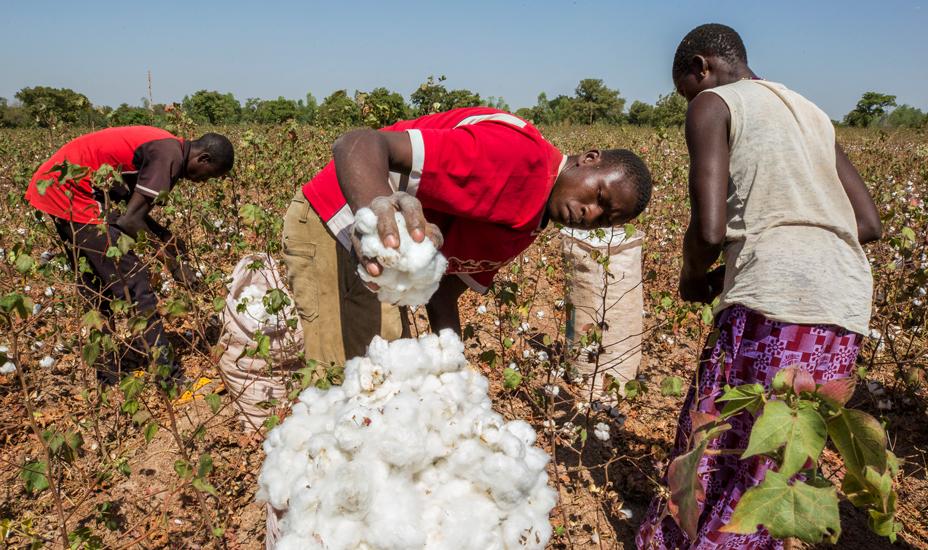
\includegraphics[keepaspectratio, height=\paperheight]{../img/cotton_farmers.jpg}};
  \end{tikzpicture}
\end{frame}
% ----------------------------------------------------
% IMAGE NEEDED: cotton_farmers.jpg -- imagen que contraste la recogida manual de algodon en Africa (p.ej., en Mali o Burkina Faso, agricultores recogiendo algodon a mano) con la produccion mecanizada de algodon en EE.UU. (grandes cosechadoras en Texas o Mississippi); o simplemente una imagen de agricultores africanos de algodon en sus campos
\note{La imagen ilustra la desigualdad en la produccion de algodon. Mientras que los productores estadounidenses utilizan maquinaria avanzada y reciben subsidios gubernamentales masivos, los agricultores africanos trabajan manualmente y compiten en un mercado mundial donde los precios estan artificialmente deprimidos por los subsidios americanos. Los paises africanos productores de algodon (Mali, Burkina Faso, Chad, Benin) han denunciado repetidamente esta situacion en la OMC, pero las negociaciones han avanzado muy lentamente. Es un caso de manual de como la politica comercial de los paises ricos afecta directamente a los mas pobres del mundo.}

% ====================================================
\section{Estrategias de desarrollo}
% ====================================================

% ----------------------------------------------------
\begin{transitionframe}
Estrategias de desarrollo
\end{transitionframe}
% ----------------------------------------------------
\note{}

% ----------------------------------------------------
\begin{frame}
\frametitle{Tres grandes estrategias}
\centering
\vspace{0.3em}

\begin{tikzpicture}[>=stealth, thick]
  % Timeline base
  \draw[thick] (0,0) -- (10,0);

  % Period bands below
  \fill[accent2!20] (0,-0.8) rectangle (4,-0.3);
  \fill[accent!25] (4,-0.8) rectangle (7,-0.3);
  \fill[asher!20] (7,-0.8) rectangle (10,-0.3);

  % Period labels
  \node[font=\scriptsize, align=center] at (2,-0.55) {ISI};
  \node[font=\scriptsize, align=center] at (5.5,-0.55) {EOI (Tigres)};
  \node[font=\scriptsize, align=center] at (8.5,-0.55) {Consenso Washington};

  % Ticks above
  \foreach \x/\lab in {0/1930s, 4/1960s, 7/1980s, 10/2000s} {
    \draw (\x, -0.1) -- (\x, 0.25);
    \node[above, font=\scriptsize] at (\x, 0.2) {\lab};
  }

  % Event labels above
  \node[above, font=\scriptsize, align=center, text=accent2] at (2, 0.5) {Proteccionismo\\Empresas estatales};
  \node[above, font=\scriptsize, align=center, text=accent] at (5.5, 0.5) {Promoci\'{o}n exportadora\\Estado desarrollista};
  \node[above, font=\scriptsize, align=center, text=asher] at (8.5, 0.5) {Liberalizaci\'{o}n\\Privatizaci\'{o}n};
\end{tikzpicture}

\vspace{12pt}
\onslide<2->{\small Tres \'{e}pocas, tres recetas diferentes --- \textquestiondown cu\'{a}l funcion\'{o}?}

\end{frame}
% ----------------------------------------------------
\note{Esta linea temporal resume las tres grandes estrategias de desarrollo que se han intentado desde mediados del siglo XX. La ISI (Industrializacion por Sustitucion de Importaciones) domino en Latinoamerica desde los anos 30 hasta los 80. La EOI (Industrializacion Orientada a la Exportacion) fue la estrategia de los tigres asiaticos desde los anos 60. El Consenso de Washington domino desde los anos 80-90 en adelante, promovido por el FMI y el Banco Mundial. Cada estrategia tiene exitos y fracasos, y el debate sobre cual es la mejor politica de desarrollo sigue vivo. Lo interesante es que las tres responden al mismo problema (como industrializarse y crecer) pero proponen soluciones muy diferentes.}

% ----------------------------------------------------
\begin{frame}
\frametitle{ISI: Sustituci\'{o}n de Importaciones}
\centering

\begin{itemize}
  \item \textbf{L\'{o}gica:} producir internamente lo que se importa
  \begin{itemize}
    \item Aranceles altos para proteger la industria nacional
    \item Empresas estatales en sectores clave
    \item Control de capitales y tipo de cambio regulado
  \end{itemize}
  \vspace{4pt}
  \item<2-> \textbf{D\'{o}nde se aplic\'{o}:} Latinoam\'{e}rica (Brasil, M\'{e}xico, Argentina), India, Turqu\'{i}a
  \vspace{4pt}
  \item<3-> \textbf{Resultado inicial:} crecimiento industrial significativo (1940s--1960s)
  \vspace{4pt}
  \item<4-> \textbf{Problemas a largo plazo:}
  \begin{itemize}
    \item Industrias ineficientes protegidas de la competencia
    \item Corrupci\'{o}n y clientelismo en las empresas estatales
    \item D\'{e}ficits cr\'{o}nicos y endeudamiento externo
    \item \alert{``Inflaci\'{o}n estructural''} en muchos pa\'{i}ses
  \end{itemize}
\end{itemize}

\end{frame}
% ----------------------------------------------------
\note{La ISI fue la estrategia dominante en Latinoamerica durante medio siglo. La idea era simple: si los terminos de intercambio perjudican a los exportadores de materias primas (tesis de Prebisch), la solucion es dejar de depender de las importaciones industriales y producirlas en casa. Para ello, se imponian aranceles altos (a veces del 100 por cien o mas) sobre las importaciones de manufacturas, se creaban empresas estatales en sectores como el acero, los automoviles, la petroquimica, y se controlaba el tipo de cambio para facilitar la importacion de maquinaria. En sus primeras decadas, la ISI tuvo exitos notables: Brasil desarrollo una industria automotriz, Mexico una industria petroquimica, Argentina una industria siderurgica. Pero con el tiempo, las industrias protegidas se volvieron ineficientes (no tenian competencia), las empresas estatales se convirtieron en instrumentos de clientelismo politico, y los deficits se financiaron con deuda externa, lo que llevo a la crisis de deuda de los anos 80.}

% ----------------------------------------------------
\begin{frame}[plain]
  \begin{tikzpicture}[remember picture, overlay]
    \node[at = (current page.center), yshift = 0cm] (cover) {%
      \includegraphics[keepaspectratio, height=\paperheight]{../img/isi_factory.jpg}};
  \end{tikzpicture}
\end{frame}
% ----------------------------------------------------
% IMAGE NEEDED: isi_factory.jpg -- fotografia de una fabrica de la era ISI en Latinoamerica, por ejemplo la linea de montaje de Volkswagen en Puebla (Mexico) o la fabrica de FIAT en Argentina en los anos 60-70, o una planta siderurgica estatal latinoamericana de la epoca; transmite la idea de industrializacion protegida
\note{Imagen de una fabrica de la epoca ISI. La industria automotriz es un buen ejemplo de la ISI: en Brasil, Volkswagen instalo su primera planta en 1953, produciendo el Beetle para el mercado interno. En Mexico, la planta de Volkswagen en Puebla (1964) producia coches exclusivamente para el mercado mexicano, protegida por aranceles que hacian prohibitivo importar vehiculos. Estas fabricas generaron empleo industrial y crecimiento, pero producian a costes mucho mas altos que la competencia internacional. Un coche producido en Mexico bajo la ISI costaba el doble o el triple que el mismo modelo en Alemania. El consumidor mexicano pagaba ese sobrecoste como un impuesto implicito a la proteccion industrial.}

% ----------------------------------------------------
\begin{frame}
\frametitle{EOI: Industrializaci\'{o}n Orientada a la Exportaci\'{o}n}
\centering

\begin{itemize}
  \item \textbf{L\'{o}gica:} industrializarse produciendo para el \textbf{mercado mundial}
  \begin{itemize}
    \item Promoci\'{o}n de exportaciones (subsidios, zonas francas)
    \item Inversi\'{o}n masiva en educaci\'{o}n y capital humano
    \item Estado activo pero orientado al mercado
  \end{itemize}
  \vspace{8pt}
  \item<2-> \textbf{Los ``Tigres Asi\'{a}ticos'':} Corea del Sur, Taiw\'{a}n, Singapur, Hong Kong
  \vspace{8pt}
  \item<3-> \textbf{Resultados espectaculares:}
  \begin{itemize}
    \item Corea del Sur: de pa\'{i}s agr\'{i}cola pobre a potencia tecnol\'{o}gica (Samsung, Hyundai, LG)
    \item Singapur: de puerto colonial a centro financiero global
    \item Crecimiento del 7--10\% anual durante d\'{e}cadas
  \end{itemize}
  \vspace{8pt}
  \item<4-> Clave: \textbf{\textcolor{accent}{Estado desarrollista}} --- no laissez-faire
\end{itemize}

\end{frame}
% ----------------------------------------------------
\note{La EOI es la estrategia opuesta a la ISI: en lugar de proteger la industria nacional de la competencia exterior, los tigres asiaticos se industrializaron compitiendo en los mercados mundiales. La diferencia crucial con el laissez-faire puro es que el Estado jugo un papel muy activo: dirigio la inversion hacia sectores estrategicos, invirtio masivamente en educacion (Corea del Sur paso de tasas de analfabetismo altas a tener una de las poblaciones mas educadas del mundo en una generacion), controlo el sistema financiero para canalizar credito barato a las empresas exportadoras, y mantuvo los salarios bajos en las primeras etapas. El Estado desarrollista asiatico combinaba disciplina de mercado (las empresas tenian que competir internacionalmente) con intervencion estatal estrategica. El resultado fue el crecimiento mas rapido y sostenido de la historia economica moderna.}

% ----------------------------------------------------
\begin{frame}[plain]
  \begin{tikzpicture}[remember picture, overlay]
    \node[at = (current page.center), yshift = 0cm] (cover) {%
      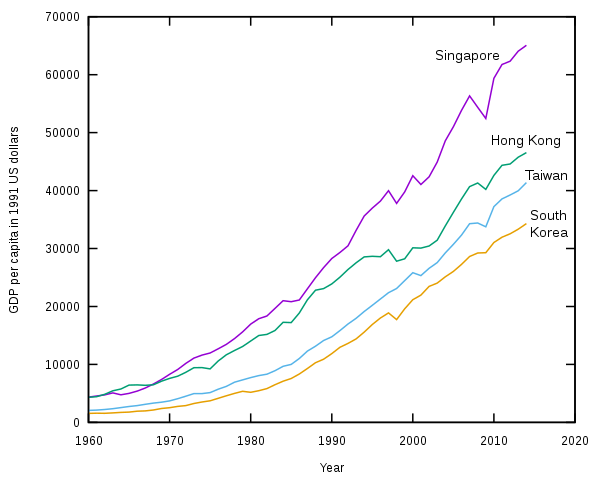
\includegraphics[keepaspectratio, height=\paperheight]{../img/asian_tigers.jpg}};
  \end{tikzpicture}
\end{frame}
% ----------------------------------------------------
% IMAGE NEEDED: asian_tigers.jpg -- skyline moderno de Seul, Singapur o Hong Kong, mostrando rascacielos y desarrollo urbano avanzado; preferiblemente una foto nocturna o panoramica que transmita modernidad y riqueza; o composicion de las cuatro ciudades (Seul, Taipei, Singapur, Hong Kong)
\note{La imagen muestra el resultado del milagro asiatico. Seul, que en los anos 50 era una ciudad devastada por la guerra, es hoy una de las ciudades mas modernas y tecnologicas del mundo. Singapur, que en 1965 era una isla pobre expulsada de la federacion malasia, tiene hoy un PIB per capita superior al de la mayoria de paises europeos. Hong Kong y Taiwan completaron transformaciones similares. Estos exitos plantearon un desafio intelectual a las teorias del desarrollo: demostraron que el subdesarrollo no es un destino, pero tambien que el crecimiento no ocurre espontaneamente: requiere politicas activas, instituciones funcionales, e inversion en capital humano.}

% ----------------------------------------------------
\begin{frame}
\frametitle{El Consenso de Washington}
\centering

\begin{itemize}
  \item A\~{n}os 1980--90: crisis de deuda en Latinoam\'{e}rica, colapso de la ISI
  \vspace{4pt}
  \item<2-> \textbf{Receta del FMI y Banco Mundial} (Williamson, 1989):
  \begin{itemize}
    \item Liberalizaci\'{o}n comercial y apertura a la inversi\'{o}n extranjera
    \item Privatizaci\'{o}n de empresas estatales
    \item Disciplina fiscal y desregulaci\'{o}n financiera
  \end{itemize}
  \vspace{4pt}
  \item<3-> \textbf{Resultados mixtos:}
  \begin{itemize}
    \item Chile: caso de ``\'{e}xito'' (pero con alto coste social inicial)
    \item Rusia, Argentina: liberalizaci\'{o}n r\'{a}pida $\rightarrow$ crisis severas
    \item \'{A}frica subsahariana: ajuste estructural con resultados pobres
  \end{itemize}
\end{itemize}

\end{frame}
% ----------------------------------------------------
\note{Consenso de Washington --- conectar con la sesion 8 (finanzas): la crisis de deuda de los 80 que vimos la sesion pasada es la que abrio la puerta al Consenso de Washington.
\begin{itemize}
  \item Nombre dado por John Williamson (1989) a las politicas que FMI, Banco Mundial y Tesoro de EE.UU. recomendaban. A veces se imponian como condicionalidad para recibir prestamos del FMI (programas de ajuste estructural).
  \item Idea central: el Estado habia intervenido demasiado y mal bajo la ISI; la solucion era liberar mercados, privatizar, abrir la economia.
  \item Chile: reformas liberales desde Pinochet en los 70, crecimiento sostenido, pero alto coste social inicial (desigualdad, represion).
  \item Rusia: liberalizacion de shock en los 90, PIB cayo un 40 por ciento, emergieron oligarcas que compraron empresas estatales a precios de ganga.
  \item Argentina: privatizaciones masivas, convertibilidad del peso en los 90, colapso de 2001 (conectar con lo visto sobre crisis monetarias en la sesion anterior).
\end{itemize}}

% ----------------------------------------------------
\begin{frame}
\frametitle{Globalizaci\'{o}n y sus descontentos}
\centering

\begin{itemize}
  \item La globalizaci\'{o}n econ\'{o}mica ha generado \textbf{ganadores y perdedores}:
  \vspace{8pt}
  \item<2-> \textbf{Ganadores:}
  \begin{itemize}
    \item China, India, Vietnam: crecimiento gracias al comercio y la IED
    \item Consumidores de pa\'{i}ses ricos: productos baratos
    \item Clases medias emergentes en Asia
  \end{itemize}
  \vspace{8pt}
  \item<3-> \textbf{Perdedores:}
  \begin{itemize}
    \item Trabajadores industriales en pa\'{i}ses ricos (\textit{China shock})
    \item Pa\'{i}ses que liberalizaron sin instituciones s\'{o}lidas
    \item Pa\'{i}ses dependientes de materias primas: vulnerabilidad a los precios
  \end{itemize}
  \vspace{8pt}
  \item<4-> \alert{Reacci\'{o}n pol\'{i}tica:} auge del populismo, proteccionismo, escepticismo ante la apertura
\end{itemize}

\end{frame}
% ----------------------------------------------------
\note{La globalizacion ha sacado a cientos de millones de personas de la pobreza (sobre todo en Asia), pero tambien ha generado perdedores claros. El China shock es un termino academico para describir el impacto de la entrada de China en la OMC (2001) sobre los trabajadores industriales de paises ricos: millones de empleos manufactureros desaparecieron en EE.UU. y Europa, concentrados en regiones especificas (el Rust Belt americano, las regiones industriales del norte de Inglaterra). Estos perdedores de la globalizacion han alimentado movimientos politicos populistas: el Brexit en el Reino Unido, la eleccion de Trump en 2016, el auge de la extrema derecha en Europa. El punto clave para el desarrollo: la globalizacion puede ser beneficiosa, pero solo si se combina con instituciones solidas y politicas de proteccion social. Sin esas condiciones, la apertura puede ser desestabilizadora.}

% ----------------------------------------------------
\begin{frame}
\centering
\vspace{2em}

{\large Dado lo que hemos visto sobre estrategias de desarrollo\ldots}

\vspace{1.5em}

{\large \textbf{\textquestiondown Qu\'{e} tipo de intervenci\'{o}n crees que ser\'{i}a m\'{a}s \'{u}til\\[0.3em]
para un pa\'{i}s pobre hoy?}}

\vspace{1em}
{\small M\'{a}s ayuda, mejores instituciones, o acceso a mercados?}

\end{frame}
% ----------------------------------------------------
\note{Segunda pausa reflexiva antes de la seccion final. Dejar que los estudiantes debatan brevemente. Las respuestas anticipan las tres posiciones del debate Sachs-Easterly-Deaton que viene a continuacion. Si los estudiantes ya tienen opiniones formadas, el debate academico que sigue les resultara mas significativo.}

% ====================================================
\section{\textquestiondown Ayuda o comercio?}
% ====================================================

% ----------------------------------------------------
\begin{transitionframe}
\textquestiondown Ayuda o comercio?
\end{transitionframe}
% ----------------------------------------------------
\note{}

% ----------------------------------------------------
\begin{frame}[plain]
  \begin{tikzpicture}[remember picture, overlay]
    \node[at = (current page.center), yshift = 0cm] (cover) {%
      \includegraphics[keepaspectratio, height=\paperheight]{../img/aid_debate.jpg}};
  \end{tikzpicture}
\end{frame}
% ----------------------------------------------------
% IMAGE NEEDED: aid_debate.jpg -- imagen relacionada con la ayuda al desarrollo: distribucion de ayuda humanitaria, reunion del Banco Mundial, o voluntarios de una ONG en un pais en desarrollo; transmite el debate sobre la eficacia de la ayuda
\note{Imagen de apertura de la ultima seccion. La ayuda al desarrollo es uno de los temas mas debatidos en la politica del desarrollo. Cada ano, los paises ricos destinan alrededor de 100.000 millones de dolares en ayuda oficial al desarrollo. Suena como mucho, pero dividido entre los miles de millones de personas pobres del mundo, son unos 20 dolares por persona. La pregunta central: sirve la ayuda para algo, o es el comercio y las instituciones domesticas lo que realmente importa.}

% ----------------------------------------------------
\begin{frame}
\frametitle{La ayuda al desarrollo: cifras}
\centering

\begin{itemize}
  \item Ayuda Oficial al Desarrollo (AOD): $\sim$\textbf{100.000 millones \$/a\~{n}o}
  \vspace{8pt}
  \item<2-> \textbf{Parece mucho, pero\ldots}
  \begin{itemize}
    \item Dividido entre la poblaci\'{o}n pobre mundial: $\sim$\textbf{20\$ por persona}
    \item Objetivo ONU: 0,7\% del PIB --- pocos pa\'{i}ses lo cumplen
    \item Mayor donante en t\'{e}rminos absolutos: EE.UU.
    \item Mayor donante en \% del PIB: pa\'{i}ses escandinavos
  \end{itemize}
  \vspace{8pt}
  \item<3-> \textbf{Problemas:}
  \begin{itemize}
    \item Motivaciones \alert{geopol\'{i}ticas}, no humanitarias
    \item Ayuda condicionada: obliga a comprar productos del donante
    \item Corrupci\'{o}n y desvío de fondos en pa\'{i}ses receptores
    \item Puede generar \textbf{dependencia}
  \end{itemize}
\end{itemize}

\end{frame}
% ----------------------------------------------------
\note{Las cifras de la ayuda al desarrollo son enganosas. 100.000 millones de dolares al ano suenan como mucho, pero es menos de lo que los europeos gastan en helados al ano. Dividido entre los miles de millones de personas que viven en la pobreza, son unos 20 dolares por persona. Ademas, mucha de esa ayuda no es realmente ayuda: incluye costes administrativos, salarios de expatriados, y ayuda atada (que obliga al pais receptor a comprar bienes y servicios del pais donante, lo que infla los costes). Las motivaciones de la ayuda tampoco son puramente humanitarias: durante la Guerra Fria, EE.UU. y la URSS daban ayuda a sus aliados independientemente de su calidad democratica. Hoy, la ayuda sigue teniendo una fuerte dimension geopolitica: Francia da ayuda a sus antiguas colonias, EE.UU. a sus aliados estrategicos (Egipto, Israel, Afganistan).}

% ----------------------------------------------------
\begin{frame}
\frametitle{El gran debate: Sachs vs.\ Easterly vs.\ Deaton}
\centering
\vspace{0.3em}

{\footnotesize
\begin{tabularx}{\textwidth}{>{\bfseries}p{2.2cm} L L L}
 & \textbf{\textcolor{accent}{Sachs}} & \textbf{\textcolor{accent2}{Easterly}} & \textbf{\textcolor{asher}{Deaton}} \\[6pt]
\hline
Posici\'{o}n & M\'{a}s ayuda & Menos ayuda & Cautela \\[5pt]
Argumento & Trampa de pobreza: sin ``gran empuj\'{o}n'' no hay salida & La ayuda crea dependencia y distorsiona incentivos & La ayuda puede hacer da\~{n}o al debilitar gobiernos \\[5pt]
Soluci\'{o}n & Duplicar la AOD & Intervenciones puntuales de mercado & Fortalecer instituciones dom\'{e}sticas \\[5pt]
Met\'{a}fora & ``El fin de la pobreza'' & ``La carga del hombre blanco'' & ``El Gran Escape'' \\[5pt]
\end{tabularx}
}

\vspace{8pt}
\onslide<2->{\small \textbf{Banerjee y Duflo} (Nobel 2019): ni gran empuj\'{o}n ni laissez-faire\\ $\rightarrow$ \textbf{\textcolor{accent}{intervenciones espec\'{i}ficas basadas en evidencia}} (ensayos aleatorizados, RCTs)}

\end{frame}
% ----------------------------------------------------
\note{El debate sobre la ayuda tiene tres grandes posiciones. Jeffrey Sachs (El fin de la pobreza, 2005) argumenta que los paises mas pobres estan atrapados en una trampa de pobreza: son demasiado pobres para invertir en infraestructura, educacion y salud, y sin esas inversiones no pueden crecer. La solucion: un gran empujon (big push) de ayuda masiva para romper la trampa. William Easterly (La carga del hombre blanco, 2006) responde que decadas de ayuda han demostrado que el dinero no resuelve el problema; la ayuda crea dependencia, distorsiona los incentivos de los gobiernos (que se orientan a complacer a los donantes en vez de a sus ciudadanos), y financia la corrupcion. Angus Deaton (El Gran Escape, 2013) adopta una posicion intermedia: la ayuda puede hacer dano cuando debilita la relacion fiscal entre gobierno y ciudadanos (si el gobierno se financia con ayuda externa, no necesita cobrar impuestos, y por tanto no necesita rendir cuentas). Banerjee y Duflo proponen una cuarta via: ni ayuda masiva ni abandono, sino intervenciones especificas (redes antimosquitos, micronutrientes, incentivos educativos) cuya eficacia se prueba con ensayos aleatorizados (RCTs).}

% ----------------------------------------------------
\begin{frame}
\frametitle{Conclusi\'{o}n: \textquestiondown qu\'{e} sabemos?}
\centering

\begin{itemize}
  \item No hay una \textbf{receta \'{u}nica} para el desarrollo
  \vspace{8pt}
  \item<2-> Los \textbf{factores dom\'{e}sticos} son fundamentales:
  \begin{itemize}
    \item Instituciones inclusivas
    \item Inversi\'{o}n en bienes p\'{u}blicos
    \item Gesti\'{o}n inteligente de los recursos
  \end{itemize}
  \vspace{8pt}
  \item<3-> El \textbf{entorno internacional} importa, pero no determina:
  \begin{itemize}
    \item Legado colonial, t\'{e}rminos de intercambio, reglas del juego
    \item Pero: Corea, Botsuana, China demuestran que se puede superar
  \end{itemize}
  \vspace{8pt}
  \item<4-> \textbf{\textcolor{accent}{Optimismo cauteloso}}: la pobreza extrema ha ca\'{i}do dr\'{a}sticamente
  \begin{itemize}
    \item Pero el progreso no es autom\'{a}tico ni uniforme
  \end{itemize}
\end{itemize}

\end{frame}
% ----------------------------------------------------
\note{La conclusion de la sesion debe transmitir que el desarrollo es un fenomeno complejo y multifactorial. No hay una sola variable que lo explique todo: ni la geografia, ni las instituciones, ni el colonialismo, ni las estrategias comerciales por si solas. Lo que si sabemos es que las instituciones domesticas (derechos de propiedad, rendicion de cuentas, inversion en bienes publicos) son probablemente el factor mas importante. El entorno internacional puede facilitar o dificultar el desarrollo, pero no lo determina: paises como Corea del Sur y Botsuana han logrado desarrollarse a pesar de condiciones iniciales adversas. La buena noticia es que la pobreza extrema ha disminuido drasticamente: de mas de la mitad de la poblacion mundial en 1981 a alrededor del 10 por ciento hoy. La mala noticia es que este progreso se concentra en unos pocos paises (China, India, sudeste asiatico) y que Africa subsahariana sigue rezagada.}

% ----------------------------------------------------
\begin{frame}[plain]
\centering
\vspace{3em}

{\Large \textquestiondown Preguntas?}

\end{frame}
% ----------------------------------------------------
\note{}
